Domain adaptation for image recognition tries to exploit the knowledge from a source domain with plentiful data to help learn a classifier for the target domain with a different distribution and little labeled training data. In domain adaptation, the source and target domains share the same label but their data are drawn from different distributions.

In domain adaptation, the knowledge of the source domain can be transferred by 3 different approaches: \textit{instance transfer}, \textit{model transfer} and \textit{feature representation transfer} \cite{pan2010survey}. In this paper, we focus on the model transfer approach. Some recent works show that exploiting the knowledge from the source model can boost the performance of the target model effectively\cite{kuzborskij2013n,tommasi2014learning}.
Moreover, in some real applications, we can only obtain the source models and it is difficult to access their training data for different reasons such as the data credential.   
Recently, a framework called Hypothesis Transfer Learning (HTL) \cite{kuzborskij2013stability} has been proposed to handle this situation. HTL assumes only source models trained on the source domain can be utilized and there is no access to source data, nor any knowledge about the relatedness of the source and target distributions. 


Previous research \cite{ben2010theory,ben2007analysis} shows that without carefully measuring the distribution similarity between the source and target data, the source knowledge could not be exploited effectively or even hurt the learning process (called  \textit{negative transfer})\cite{pan2010survey}. 
However, as we are not able to access the source data in an HTL setting, how to effectively and safely exploit the knowledge from the source model could be an important issue in HTL, especially when target data is relatively small (Effectiveness issue). Moreover, the source models from different domains can be trained with different kinds of classifiers. For example most models trained from ImageNet are deep convolutional neural networks while some models of the VOC recognition task could be SVMs or ensemble models. Therefore, a practical HTL algorithm should be compatible with different types of source classifiers (Compatibility issue). Previous work is limited to either leveraging the knowledge from certain type of source classifiers \cite{tommasi2014learning,fei2006one} or low transfer efficiency in a small training set\cite{jie2011multiclass}. To the best of our knowledge, none of the previous work in HTL is able to solve these two issues at the same time.

In this paper, we propose our method, {called Effective Multiclass Transfer Learning (EMTLe)}, that can solve these two issues simultaneously. 
%Previous work such as MKTL \cite{jie2011multiclass} suggests that using the prediction of the source model as the transferable knowledge can greatly increase the compatibility of the transfer model for the HTL problem. However, MKTL uses a complex transfer strategy which makes it inefficient for small target training set. 
In this paper, we introduce our strategy that uses the class prediction of the source model as the transferable knowledge to help the classification. Specifically, we use the weighted class probabilities produced by the source models to adjust the prediction from the target model. Here we call the weight of each source model \textit{transfer parameter} which essentially controls the amount of knowledge transferred from the specific model. Moreover, compared to the previous work such as MKTL \cite{jie2011multiclass}, EMTLe has fewer hyperparameters to estimate. Therefore, it is easier for EMTLe to learn a good target model especially on a small training set. %We argue that the transfer parameter is a hyperparameter of our model and cannot be solved directly.

%\begin{figure}
%	\centering
%	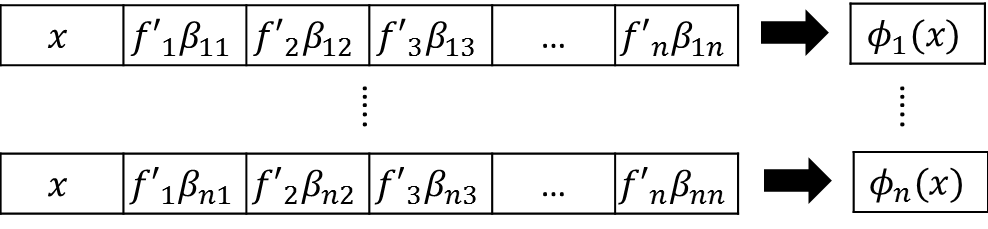
\includegraphics[scale=0.5]{fig/mktl.png}
%	\caption{Illustration of MKTL. $f_i'$ is the output of the $i$-th source model and $\beta_{in}$ is the hyperparameter (need to be estimated) to weigh the source knowledge. $Y_n$ is the decision of the $n$-th binary model.}
%	\label{fig:mktl}
%\end{figure}

To estimate the transfer parameter, we introduce bi-level optimization\cite{Pedregosa16}, which has been widely used for many different hyperparameter optimization problems recently. Specifically, on the low-level optimization problem, we use a least-square SVMs to train a model on the target data and on the high level, we introduce our novel multi-class hinge loss with $\ell_2$ penalty that can better estimate the transfer parameter when training set is small. Moreover, we show that our bi-level optimization transfer parameter estimation problem is a strongly convex optimization problem and demonstrate that our method EMTLe can find the $O({\log(t)}/{t})$ optimal solution with $t$ iterations. 

We perform comprehensive experiments on 4 real-world datasets from two benchmark datasets (3 from Office and 1 from Caltech256). We show that EMTLe can effectively transfer the knowledge with different types of source models and outperforms the baseline methods under the HTL setting. %Moreover, we show that our novel high level objective function with $\ell_2$ penalty can improve the performance of the target model effectively when the size of the training data is small. 

%The rest of this paper is organized as follows: In Section \ref{sec:work} we introduce the issues in transfer learning and some related work regarding these issues.
%In Section \ref{sec:prob}, we introduce our strategy using the class probabilities as the auxiliary bias to adapt different types of source models.
%Then, we propose a novel objective function using $\ell_2$ penalty term for transfer parameter estimation, called EMTLe in Section \ref{sec:smitle}. We use bi-level hyperparameter optimization to estimate the transfer parameter. 
%In Section \ref{sec:exp}, we show the performance comparison between EMTLe and other baselines on 4 real-world datasets.
